\section{Packet Error Probability}\label{sec:pep}
Now that we are able to simulate the \gls{rssi} when transmitting from one node to another, we need to be able to simulate whether the packet should arrive on the receiving node. With wireless radio communication, there is a chance that a receiving node may not receive the entire packet correctly, which is why we need some way of computing the probability of this happening. For this, we introduce the packet error probability. The computations in this section are derived from \cite{massoud2007digital}, as well as personal communication with the author of \cite{paper:linkmodel}. \medbreak

\subsection{Radio Model}

First we calculate the noise power $P_{N,db} = thermal\_noise + noise\_figure$ in \acrshort{db}. The noise power is calculated with the thermal noise and noise figure, and is the level of background noise affecting the wireless radio communication. For the Reachi devices we assume that the

$thermal\_noise = -119.66$ \acrshort{db} and the $noise\_figure = 4.2$ \acrshort{db}. \medbreak

Next we need to add the noise from interfering transmissions happening at the same time. We do this by adding the sum of the \gls{rssi} from interfering transmitters to the noise power $P_{N,dB}$, giving us $P_{NI,dB}$ on the link between the receiving node $n_r$ and the transmitting node $m_t$. The set of currently transmitting nodes are denoted by $nodes_t$ and the function $RSSI_{dBm}(n, m)$ denotes the RSSI on the link between nodes $n$ and $m$.
\begin{eq}\label{eq:noisepower}
    P_{NI,db}(n_r, m_t, nodes_t) = 10 \log_{10}\left( 10^{\frac{P_{N,dB}}{10}} + \mathlarger{\sum}\limits_{m \in nodes_t - \{m_t\}}  10^{\frac{RSSI_{dBm}(n_{r}, m)}{10}} \right)
\end{eq}

Note that as both the noise power $P_{N,dB}$ and the \gls{rssi} is in \acrshort{db} (a logarithmic scale), we first need to convert the values to linear scale, before computing the sum of the noise and interference power, and then convert the value back into logarithmic scale (\acrshort{db}). \smallbreak

Next we calculate the signal to noise (and interference) ratio $\gamma_{dB}$ in \acrshort{db}. The ratio $\gamma_{dB}$ is the ratio between signal and noise, that compares the level of the signal to the level of the background noise (including the interference from other transmissions), and is computed by subtracting the noise power $P_{NI,db}$:

%We expand upon this further to include the interference of other transmissions happening at the same time. This is done by computing the \gls{rssi} from interfering transmitters, and subtracting this from the \gls{sinr}, which gives us the \acrlong{snir}:

% n receiver, m transmitter

%where we assume that the $thermal\_noise = -119.66$ \acrshort{db} and the $noise\_figure = 4.2$ \acrshort{db}.

%\begin{eq}
%    P_{N,db} = thermal\_noise + noise\_figure
%\end{eq}

%Signal to noise ratio with interference, on a link from $n_r$ (receiver) to $n_t$ (transmitter). The set of currently transmitting nodes are denoted by $nodes_t$. The function $RSSI(n, m)$ denotes the RSSI on the link between nodes $n$ and $m$. We subtract the sum of the RSSI between $n_r$ and any currently transmitting nodes, excluding $m_t$.

\begin{eq}
    \gamma_{dB}(n_r, m_t, nodes_t) = RSSI(n_r, m_t) - P_{NI,dB}(n_r, m_t, nodes_t)
\end{eq}

We use this to compute the bit error probability $P_b$:

%\begin{eq}
%    \gamma = 10^{\frac{\gamma_{dB}}{10}}
%\end{eq}

\begin{eq}
    P_b(n_r, m_t, nodes_t) = \frac{1}{2}erfc \left( \sqrt{ \left( \frac{10^{\frac{\gamma_{dB}(n_r, m_t, nodes_t)}{10}}}{2} \right)} \right)
\end{eq}

which we finally can use to compute the packet error probability $P_p$. The packet error probability is the probability that we experience a bit error for any of the bits in our packet, during transmission.
\begin{eq}
    P_p(n_r, m_t, nodes_t, packetsize) = 1 - \left( 1 - P_b(n_r, m_t, nodes_t) \right) ^{packetsize}
\end{eq}


\subsection{Example}
In \autoref{sec:linkmodel}, we computed the link model for a sample network topology \textbf{G}. \autoref{eq:rssivector} shows a vector containing the \gls{rssi}, in \acrshort{dbm}, for each of the six links in the network, assuming a transmission power of 26 \acrshort{dbm}. For the following, it is assumed that $thermal\_noise = -119.66$ \acrshort{db}, the $noise\_figure = 4.2$ \acrshort{db}, and $packetsize = 160$ bits (which is the size of a header packet for the Reachi devices).

\begin{eq}\label{eq:rssivector}
    \vect{RSSI_{dBm, \textbf{G}}} =
    \begin{bmatrix}
        -67.390 \\
        -61.734 \\
        -72.170 \\
        -52.163 \\
        -74.042 \\
        -72.413
    \end{bmatrix}
\end{eq}

If we assume that $n_2$ is currently listening, and the currently transmitting nodes $nodes_t = \{n_1, n_4\}$. What is the probability for packet error on the link between nodes $n_2$ and $n_1$ with interference from node $n_4$? First, we compute the noise power $P_{NI,db}$, according to \autoref{eq:noisepower}:
\begin{eq}
    P_{NI,db}(n_2, n_1, nodes_t) = 10 \log_{10}\left( 10^{\frac{(-119.66 + 4.2)}{10}} + 10^{\frac{-74.042}{10}} \right) = -74.041
    %\mathlarger{\sum}\limits_{m \in {n_1, n_3}}  10^{\frac{RSSI_{dBm}(n_{2}, m)}{10}} [m \neq n_{4}] \right) 
\end{eq}

We subtract the noise power $P_{NI,db}$ from the \gls{rssi} to get the signal to noise (and interference) ratio $\gamma_{dB}$:
\begin{eq}
    \gamma_{dB}(n_2, n_1, nodes_t) = -67.390 - (-74.041) = 6.651
\end{eq}

With which we can compute the bit error probability:
\begin{eq}
    P_b(n_2, n_1, nodes_t) = \frac{1}{2}erfc \left( \sqrt{ \left( \frac{10^{\frac{6.651}{10}}}{2} \right)} \right) = 0.000536
\end{eq}

Finally we can compute the packet error probability using the bit error probability:
\begin{eq}
    P_p(n_2, n_1, nodes_t, packetsize) = 1 - \left( 1 - 0.000536 \right) ^{160} = 0.082
\end{eq}

This gives us a 8.2 \% probability that we will experience packet error on the link from $n_2$ to $n_1$, with a single interfering transmitter, which is a significant difference in relation to the same transmission with no interfering transmitters. To demonstrate this, \autoref{figure:pepegraph} shows the probability for packet error with no interfering transmitters. According to the figure, an \gls{rssi} of approximately $-103.0$ \acrshort{dbm} would have a probability for packet error close to zero, and an \gls{rssi} of approximately $-110.0$ \acrshort{dbm} would have a probability for packet error close to 100 \%. If we look back to the \gls{rssi} vector, \vect{RSSI_{dBm, \textbf{G}}}, we see that the \gls{rssi} on the link between nodes $n_1$ and $n_2$ is $-67.390$ \acrshort{dbm}, which is significantly better than the $-103.0$ \acrshort{dbm} we see in the graph, but with just a single interfering transmitter, the probability for packet error increases to 8.2 \%, which corresponds to what we see in \autoref{figure:pepegraph1}, where an \gls{rssi} of approximately $-66.0$ \acrshort{dbm} is required for a probability for packet error close to zero, with a single interfering transmitter.

%\begin{figure}[H]
%    \centering
%    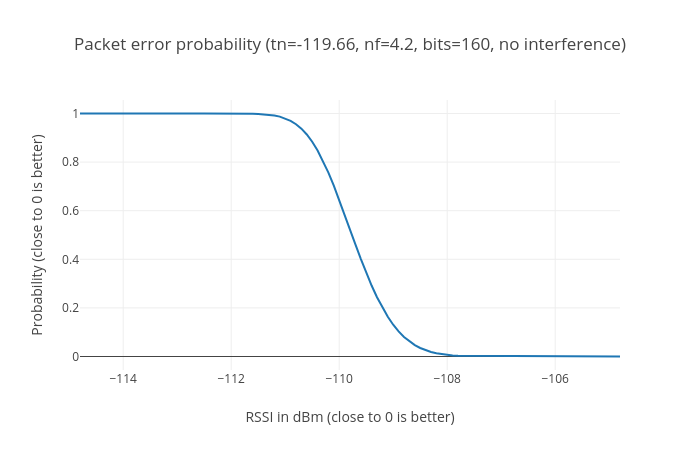
\includegraphics[width=.8\textwidth]{figures/pep/pep_0_interference.png}
%    \caption{Probability for packet loss on a link with no interfering transmitters.}
%    \label{figure:pepegraph}
%\end{figure}
%\begin{figure}[H]
%    \centering
%    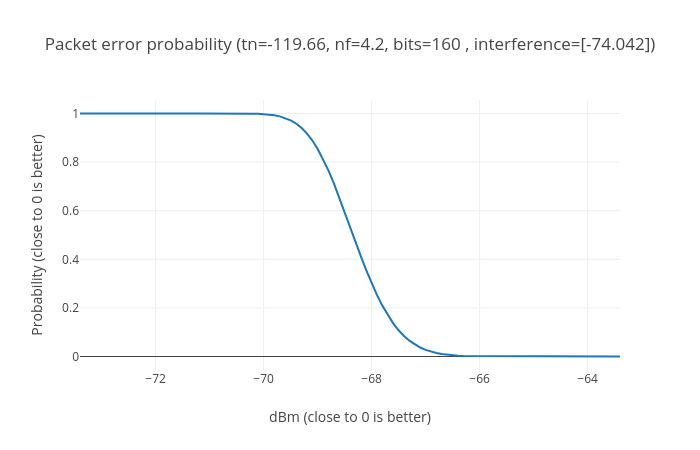
\includegraphics[width=.8\textwidth]{figures/pep/pep_1_interference.png}
%    \caption{Probability for packet loss on a link with a single interfering transmitter.}
%    \label{figure:pepegraph1}
%\end{figure}
\begin{figure}[H]
    \centering
    \begin{subfigure}[t]{.9\textwidth}
        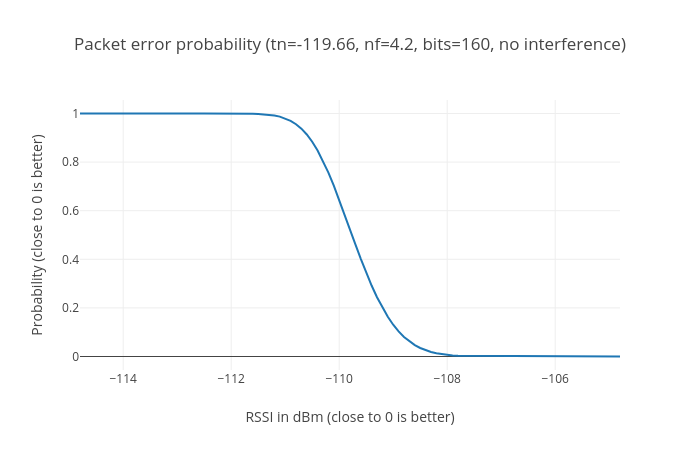
\includegraphics[width=\linewidth]{figures/pep/pep_0_interference.png}
        \caption{Probability for packet error on a link with no interfering transmitters.}
        \label{figure:pepegraph}
    \end{subfigure}
    \begin{subfigure}[t]{.9\textwidth}
        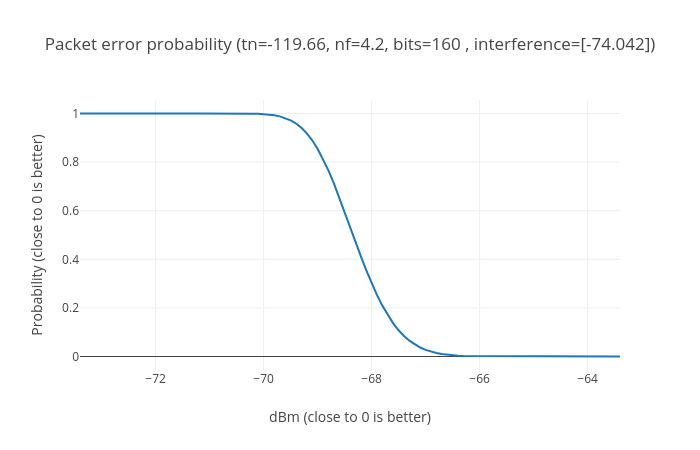
\includegraphics[width=\linewidth]{figures/pep/pep_1_interference.png}
        \caption{Probability for packet error on a link with a single interfering transmitter.}
        \label{figure:pepegraph1}
    \end{subfigure}
    \caption{Probability for packet error with and without interfering transmitters.}
    \label{figure:pepegraphs}
\end{figure}

%Compared to the \gls{rssi} on the link between $n_1$ and $n_2$, 

%If we assume that $n_2$ is currently listening, and the currently transmitting nodes are $nodes_t = {n_1, n_3, n_4}$. Now, we want to compute the probability for packet error on the link between nodes $n_2$ and $n_4$.

%\subsection*{Example}
%
%\begin{figure}[H]
%    \centering
%    \begin{tikzpicture}
%        \begin{scope}[xshift=4cm]
%        \node[main node] (1) {$1$};
%        \node[main node] (2) [left = 2cm  of 1]  {$2$};
%        \node[main node] (3) [below = 2cm  of 2] {$3$};
%        \node[main node] (4) [right = 2cm  of 3] {$4$};
%
%        \path[draw,thick]
%        (1) edge node[above] {$l_1$} (2)
%        (1) edge node[above=.8cm, right] {$l_2$} (3)
%        (1) edge node[right] {$l_3$} (4)
%        (2) edge node[left] {$l_4$} (3)
%        (2) edge node[below=.8cm, right] {$l_5$} (4)
%        (3) edge node[below] {$l_6$} (4)
%        ;
%        \end{scope}
%    \end{tikzpicture}
%    \caption{Sample graph \textbf{G} with 4 nodes and 6 links.}
%    \label{figure:lm-sample}
%\end{figure}
%

%The vector \vect{RSSI_{\textbf{G}}} contains the RSSI for all links in \textbf{G}. It is assumed that $thermal\_noise = -119.66$ \acrshort{db}, the $noise\_figure = 4.2$ \acrshort{db}, and $packetsize = 160$. \medbreak

%If we assume that $n_2$ is currently listening, and the currently transmitting nodes are $nodes_t = {n_1, n_3, n_4}$. Now, we want to compute the probability for packet error on the link between nodes $n_2$ and $n_4$.
%(-119.66 + 4.2)
%\begin{eq}
%    \gamma_{dB}(n_2, n_4) = RSSI(n_2, n_4) - P_{N,dB} - \mathlarger{\sum}\limits_{m \in \{n_1, n_3, n_4\}} RSSI(n_2, m)[m \neq n_4]
%\end{eq}
%
%\begin{eq}
%    \gamma_{dB}(n_2, n_4) = -74.042 - (-119.66 + 4.2) - (-64.610 + (-52.163)) = 158.191
%\end{eq}
%
%\begin{eq}
%    P_b(n_2, n_4) = \frac{1}{2}erfc \left( \sqrt{ \left( \frac{10^{\frac{158.191}{10}}}{2} \right)} \right) = 1.406 %\cdot 10^{-36}
%\end{eq}
%
%\begin{eq}
%    P_p(n_2, n_4) = 1 - \left( 1 - P_b(n_2, n_4) \right) ^{160} = 0.0
%\end{eq}

%Which equals to a probability of approximately 10 \% packet loss, with no interference, and an \gls{rssi} of $-105.3$ \acrshort{dbm}.
